\documentclass[11pt]{article}
\usepackage[sc]{mathpazo} %Like Palatino with extensive math support
\usepackage{amsmath}
\usepackage{fullpage}
\usepackage[authoryear,sectionbib,sort]{natbib}
\linespread{1.7}
\usepackage[utf8]{inputenc}
\usepackage{lineno}
\usepackage{titlesec}
\usepackage{graphicx}
\titleformat{\section}[block]{\Large\bfseries\filcenter}{\thesection}{1em}{}
\titleformat{\subsection}[block]{\Large\itshape\filcenter}{\thesubsection}{1em}{}
\titleformat{\subsubsection}[block]{\large\itshape}{\thesubsubsection}{1em}{}
\titleformat{\paragraph}[runin]{\itshape}{\theparagraph}{1em}{}[. ]

\titleformat{\paragraph}[runin]{\itshape}{\theparagraph}{1em}{}[. ]\renewcommand{\refname}{Literature Cited}
\usepackage{setspace}
\usepackage{fancyhdr}
\pagestyle{fancy}
\renewcommand{\theequation}{S\arabic{equation}}
\renewcommand{\thefigure}{S\arabic{figure}}
\renewcommand{\thesection}{S\arabic{section}}
% \renewcommand{\thesubsection}{S\arabic{subsection}}

%%%%%%%%%%%%%%%%%%%%%
% Header
%%%%%%%%%%%%%%%%%%%%%
%
% Customize the line below with the last name of your first author and
% the short title of your MS. You can comment authorship information out
% while your MS is undergoing double-blind review.
%
\rhead{Supplement to ``Correlated movements reshape spatio-temporal disease dynamics'' \textit{Am.~Nat.}}
\setlength{\headsep}{0.3in}
\lhead{}

%%%%%%%%%%%%%%%%%%%%%
% Line numbering
%%%%%%%%%%%%%%%%%%%%%
%
% Please use line numbering with your initial submission and
% subsequent revisions. After acceptance, please turn line numbering
% off by adding percent signs to the lines %\usepackage{lineno} and
% to %\linenumbers{} and %\modulolinenumbers[3] below.
%
% To avoid line numbering being thrown off around math environments,
% the math environments have to be wrapped using
% \begin{linenomath*} and \end{linenomath*}
%
% (Thanks to Vlastimil Krivan for pointing this out to us!)

\title{Online Supplement: Correlated host movements can reshape spatio-temporal disease dynamics: modeling the contributions of space use to transmission risk using movement data \\
% \LaTeX{} Template for Author-Supplied Supplementary PDFs, \\
\textit{The~American~Naturalist} }

% This version of the LaTeX supplementary template was last updated on
% November 8, 2019.

%%%%%%%%%%%%%%%%%%%%%
% Authorship
%%%%%%%%%%%%%%%%%%%%%
% Please remove authorship information while your paper is under review,
% unless you wish to waive your anonymity under double-blind review. You
% will need to add this information back in to your final files after
% acceptance.
%
% Once accepted for publication, author-supplied PDFs should have a
% title page that includes (at least) the authors' names, the title of
% the MS, and the name of the journal. It should also have a header and
% page numbers.

% \author{Juan S. Vargas Soto$^{1}$ \\
% Justin Kosiewska$^{1}$ \\
% Lisa I. Muller$^{1}$ \\
% Dan Grove$^{1}$ \\
% Dailee Metts$^{1}$ \\
% Mark Q. Wilber$^{1, \ast}$
% }

\date{}

\begin{document}

% \doublespacing
\linenumbers

\section*{Appendix 0: A derivation of MoveSTIR}

The full derivation of MoveSTIR is provided in \cite{Wilber2022}. The text below is taken directly from \cite{Wilber2022} and is used to 

MoveSTIR begins from a simple compartmental host-parasite model that tracks \textbf{S}usceptible and \textbf{I}nfected host density and the density of the \textbf{P}athogen in the environment. We make the following assumptions: i) the force of infection (FOI) experienced by a susceptible host is a linear function of pathogen density in the environment $\beta P$, where $\beta$ is the transmission rate that combines rates of acquisition and contact, ii) infected hosts deposit pathogen at rate $\lambda$, iii) the pathogen decays in the environment at rate $\nu$, iv) the pathogen is well-mixed in the area where contact and acquisition occur, and v) the infection process does not substantially deplete the pathogen in the environment \citep{Dwyer1997a,Fenton2015}.  These assumptions provide a reasonable starting point for MoveSTIR but can be readily adjusted to account for non-linear FOI or extended to account for states such as \textbf{E}xposed and \textbf{R}ecovered. For simplicity, we also assume that \textbf{I}nfected hosts recover at rate $\gamma$ and are immediately \textbf{S}usceptible.

The following equations describe the infection dynamics in a host population

\begin{equation}
    \begin{aligned}
        \frac{d S}{dt} &= - \beta P S + \gamma I  \\
        \frac{d I}{dt} &= \beta P S - \gamma I \\
        \frac{d P}{dt} &= \lambda I - \nu P
     \end{aligned}
     \label{eq:base_model}
\end{equation}
where we initially assume a constant population size of $S + I = N$ and no births or deaths. Equation \ref{eq:base_model} is applicable to both microparasites (e.g., bacteria and viruses) or macroparasites (e.g., helminths) with a simple life cycle \citep[e.g.,][]{Fenton2015}.

We can equivalently express equation \ref{eq:base_model} as a renewal equation \citep{VandenDriessche2002}, namely

\begin{equation}
    \begin{aligned}
        \frac{d S(t)}{dt} &= - \beta P(t) S(t) + \gamma I(t) \\
        \frac{d I(t)}{dt} &= \beta P(t) S(t) - \gamma I(t) \\
        P(t) &= P_0(t) +  \int_{0}^{t} \lambda I(u) e^{-\nu(t - u)} du
     \end{aligned}
     \label{eq:ghosts}
\end{equation}

In equation \ref{eq:ghosts}, $I(u)$ gives the density of infected individuals at some previous time $u$, $u < t$. The function $e^{-\nu(t - u)}$ defines the pathogen survival function in the environment, assuming that the pathogen decays at a constant rate $\nu$. We could readily replace $e^{-\nu(t - u)}$ with any survival function reflective of the pathogen of interest. The parameter $P_0(t)$ is the density of pathogen present at time 0 that are still present at time $t$.

We can then substitute in the expression of $P(t)$ to re-write $\frac{d I(t)}{dt}$ as a function of $I(u)$

\begin{equation}
    \frac{d I(t)}{dt} = S(t) \beta \int_{0}^{t} \lambda I(u) e^{-\nu(t - u)} du  - \gamma I(t)
    \label{eq:base_renewal}
\end{equation}
where we assume $P_0(t) = 0$.

The function $h(t) = \beta \int_{0}^{t} \lambda I(u) e^{-\nu(t - u)} du$ is the per capita FOI at time $t$.  The FOI $h(t)$ is a rate with units time\textsuperscript{-1}. As such, $h(t)$ defines the FOI felt by an individual at a given moment after accounting for the time-dependent accumulation and decay of all pathogens previously deposited by infected hosts. Importantly, $h(t)$ lets deposition rate ($\lambda$) and contact formation and acquisition of the pathogen (both encapsulated in $\beta$) vary independently, and allows for a continuum between direct contact (when $u \approx t$) and indirect contact (when $u < t$).  However, equation \ref{eq:base_renewal} does not i) clearly separate contact formation and pathogen acquisition, ii) explicitly account for contact duration, or iii) account for directional differences in transmission risk due to the order of when individuals visit locations.  We extended equation \ref{eq:base_renewal} to consider directional interactions occurring at the individual level.

\subsection*{A pairwise view of the force of infection (FOI)}

Consider a single individual $i$ moving through space.   At each moment, the individual experiences a FOI dependent upon the full history of infected individuals that previously or presently share its current location.  Let $I(u, x)$ be the number of infected hosts in location $x$ at time $u$.  If there are $N - 1$ other hosts in the population, we can write $I(u, x) = \sum_{j = 1}^{N - 1} \delta_{x_j(u)}(x) \delta_{I_j(u)}(I)$. The function $\delta_{x_j(u)}(x)$ is an indicator function that is defined as 

\begin{equation*}
    \delta_{x_j(u)}(x) = 
    \begin{cases}
        1 &  \text{if the location of host $j$ at time $u$ is $x$ (i.e., $x_j(u) = x$)} \\
        0 & \text{otherwise}
    \end{cases}
\end{equation*}
Similarly, $\delta_{I_j(u)}(I)$ is the indicator function 

\begin{equation*}
    \delta_{I_j(u)}(I) = 
    \begin{cases}
        1 &  \text{if host $j$ is infected at time $u$ (i.e., $I_j(u) = I$)} \\
        0 & \text{otherwise}
    \end{cases}
\end{equation*}
Taken together, this means that host $j$ at past time $u$ only gets ``counted'' toward the FOI experienced by focal host $i$ at time $t$ if they are infected and shedding pathogen ($I_j(u) = I$) at time $u$ and in the same location $x$ ($x_j(u) = x$).

We can then update $h(t)$ to consider the contributions from other individual hosts to the FOI felt by a focal host $i$ at time $t$ in location $x$.

\begin{equation}
    \begin{aligned}
    h_i(t, x) &= \beta' \int_{0}^{t} \sum_{j = 1}^{N - 1} \lambda \delta_{x_j(u)}(x) \delta_{I_j(u)}(I) e^{-\nu(t - u)} du \\ &=  \underbrace{\sum_{j = 1}^{N - 1}}_{\text{Sum over individuals}} \int_{0}^{t} \underbrace{\beta'}_{\text{Acquisition}} \underbrace{\delta_{x_j(u)}(x)}_{\text{Contact}} \underbrace{\lambda \delta_{I_j(u)}(I)}_{\text{Deposition}} \underbrace{e^{-\nu(t - u)}}_{\text{Pathogen decay}} du
    \end{aligned}
    \label{eq:h_partitioned}
\end{equation}
where $\beta'$ is now an acquisition rate (i.e., an uptake rate times per pathogen probability of infection) as we have conditioned on contact with the term $\delta_{x_j(u)}(x)$.  Consider a single term in the summation, $h_{i \leftarrow j}(t, x) = \int_{0}^{t} \beta' \delta_{x_j(u)}(x) \lambda \delta_{I_j(u)}(I) e^{-\nu(t - u)} du$. We can define this term as: the FOI felt by individual $i \neq j$ at time $t$ in location $x$ due to individual $j$'s previous infection history in location $x$, up to time $t$. This quantity is a rate with units time$^{-1}$ and encapsulates pathogen acquisition, contact formation, pathogen deposition, and direct and indirect transmission. Contact duration is explicitly accounted for by the integral over $\delta_{x_j(u)}(x)$, which specifies how long host $i$ is in contact with host $j$ in the past (indirect) or present (direct). Finally, we can more explicitly account for the area of location $x$ by re-writing $\beta' \delta_{x_j(u)}(x)$ as $\tilde{\beta} \Phi(x_j(u), x)$ \citep{Gurarie2013,Martinez-Garcia2020}, where $\tilde{\beta}$ has units $\frac{\text{area units}}{\text{time}}$ (e.g., $\frac{m^2}{\text{hour}}$).  The function $\Phi(x_j(u), x)$ is the contact function and is a probability density function that integrates to one over the spatial domain of interest with units $1 / \text{area units}$ \citep[Appendix S1;][]{Gurarie2013}.

\section*{Appendix A: PMoveSTIR in continuous space}

In the main text, we derive PMoveSTIR assuming that hosts are moving and contacting each other within some area $A_x$, which we can conceptually think about as a grid cell on a gridded landscape.  While this conceptually simplifies the problem, it is more general to consider the case of continuous space where we define contact as potentially happening when present or past host $j$ is (was) within some distance $r$ of host $i$ at its present location \citep{Wilber2022}.  The output we want from this alternative version of PMoveSTIR is the function $\hat{h^*}(x, t)$, which is the force of infection \emph{per unit area} at point $x$ on the landscape (e.g., $\hat{h^*}(x, t)$ might have units day$^{-1}\text{m}^{-2}$).  Integrating this function over different areas will yield estimates of force of infection felt by host $i$ from host $j$ for any area of interest on the landscape.

Let's start with the situation where a host $i$ is occupying some circular area $A_{x, \rho}$ where $x$ is the center of the area and $\rho$ is the radius of the area.  A contact can occur when host $j$ (past or present) is in the area $A_{x, \rho + r}$ where $r$ is our epidemiologically relevant contact distance and $r >> \rho$.  The force of infection felt by host $i$ from host $j$ as time $t$ in area $A_{x, \rho}$ is given by

\begin{equation}
    h_{i \leftarrow j}(t, A_{x, \rho}) = \int_{-\infty}^{t} \beta' \lambda \delta'_{x_i(t)}(A_{x, \rho}) \delta'_{x_j(u)}(A_{x, \rho + r}) e^{-\nu(t - u)} du.
    \label{eq:prob_foi}
\end{equation} 
where, consistent with the main text, $\delta'_{x_i(t)}(A_{x, \rho})$ is a Bernoulli random variable that determines whether or not host $i$ is located in area $A_{x, \rho}$ at time $t$ and $\delta'_{x_j(u)}(A_{x, \rho + r})$ is a Bernoulli random variable that determines whether or not host $j$ is in area $A_{x, \rho + r}$ at time $u$.  The variables $x_i(t)$ and $x_j(u)$ indicate the locations of host $i$ and $j$ at time $t$ and $u$, respectively.  The parameter $\beta' = \frac{\tilde{\beta}}{A_{x, \rho + r}}$ and indicates our assumption that encounters are equally likely within an area $A_{x, \rho + r}$. The parameter $\lambda$ is the pathogen shedding rate of host $j$ and $\nu$ is the pathogen decay rate once deposited in the environment.  As in the main text, we are computing maximum transmission risk and assuming that host $j$ is always infected at any time $u$.

As we did in the main text, we can envision simulating many different movement trajectories for host $i$ and $j$ and take the expectation of $h_{i \leftarrow j}(t, A_{x, \rho})$.  We obtain

\begin{equation}
    h^*_{i \leftarrow j}(t, A_{x, \rho}) = \int_{-\infty}^{t} \beta' \lambda E[\delta'_{x_i(t)}(A_{x, \rho}) \delta'_{x_j(u)}(A_{x, \rho + r})] e^{-\nu(t - u)} du.
    \label{eq:prob_foi2}
\end{equation} 

We can rewrite equation \ref{eq:prob_foi2} as

\begin{equation}
    \begin{aligned}
        h^*_{i \leftarrow j}(t, A_{x, \rho})  = \frac{\tilde{\beta}}{A_{x, \rho + r}} \lambda \int_{-\infty}^{t} [p_i(A_{x, \rho}, t) p_j(A_{x, \rho + r}, u) + Cov(\delta'_{x_i(t)}(A_{x, \rho}), \delta'_{x_j(u)}(A_{x, \rho + r}))] e^{-\nu(t - u)} du,
    \end{aligned}
    \label{eq:correlated_movement}
\end{equation}
where the force of infection felt by host $i$ from host $j$ is the related to the utilization distributions of the two hosts and their covariance within an area (in actuality, two nested areas).  

For simplicity, consider hosts moving independently. In this case, we can write

\begin{equation}
    h^*_{i \leftarrow j}(t, A_{x, \rho}) = \beta' \lambda \int_{-\infty}^{t} [p_i(A_{x, \rho}, t) p_j(A_{x, \rho + r}, u)] e^{-\nu(t - u)} du
    \label{eq:ind_movement}
\end{equation}
where $p_i(A_{x, \rho}, t)$ is the probability of host $i$ being in area $A_{x, \rho}$ at time $t$ and $p_j(A_{x, \rho + r}, u)$ is the probability of host $j$ being in area $A_{x, \rho + r}$ at time $u$.

Now we want to calculate $h^*_{i \leftarrow j}(t, A_{x, \rho})$ in the limit as $\rho \rightarrow 0$. For equation \ref{eq:ind_movement}, we can divide both sides by $A_{x, \rho}$ and take the limit as $\rho \rightarrow 0$ (such that $A_{x, \rho} \rightarrow 0$). Doing this we obtain

\begin{equation}
    \hat{h}^*_{i \leftarrow j}(t, x) = \beta' \lambda \int_{-\infty}^{t} [f_i(x, t) p_j(A_{x, r}, u)] e^{-\nu(t - u)} du = \beta' \lambda \int_{-\infty}^{t} [f_i(x, t) \int_{y \in A_{x, r}} f_j(y, u) dy] e^{-\nu(t - u)} du
    \label{eq:limit}
\end{equation}
where $f_i(x, t)$ and $f_j(x, t)$ are the probability density functions of space use for host $i$ and host $j$, respectively.  Note that the units on $f_i(x, t)$ or $f_j(x, t)$ are per area, such that the force of infection $\hat{h}^*_{i \leftarrow j}(t, x)$ has units per time per area as opposed to $h^*_{i \leftarrow j}(t, A_{x, \rho})$ which has units per time. Conceptually, for $h^*_{i \leftarrow j}(t, A_{x, \rho})$ we have already integrated over area so we cancel out the per area units.  

Assuming a stationary process, we can write equation \ref{eq:limit} as

\begin{equation}
    \hat{h}^*_{i \leftarrow j}(t, x) =  \frac{\beta' \lambda}{\nu} [f_i(x) \int_{y \in A_{x, r}} f_j(y) dy]
\end{equation}

Furthermore, if we assume that the space use of host $j$ is relatively uniform within the contact area $A_{x, r}$ we can simplify to

\begin{equation}
    \hat{h}^*_{i \leftarrow j}(t, x) =  \frac{\beta' \lambda}{\nu} [f_i(x) f_j(x) \pi r^2]
\end{equation}

Remembering that $\beta' = \tilde{\beta} / A_{x, r} = \tilde{\beta} / \pi r^2$, we get 

\begin{equation}
    \hat{h}^*_{i \leftarrow j}(t, x) =  \frac{\tilde{\beta} \lambda}{\nu} [f_i(x) f_j(x)]
\end{equation}

Integrating $\hat{h}^*_{i \leftarrow j}(t, x)$ over some area of interest centered at $x$ would yield  $h^*_{i \leftarrow j}(t, A_{x, r}) = \frac{\tilde{\beta} \lambda}{\nu} \int_{A_{x, r}} [f_i(y) f_j(y) dy] $. This is reminiscent of the equation 17 in \cite{Martinez-Garcia2020} where a limiting case of the mean encounter rate of two individuals moving according to an Ornstein-Uhlenbeck movement process is proportional to the inner product of their utilization distributions. 

Including correlation in movement into this formulation of PMoveSTIR is more theoretically and empirically challenging, and we leave this task for a later paper.

\section*{Appendix B: Deriving PMoveSTIR given an assumption of statistical stationarity}

To derive equation 5 in the main text that assumes stationarity in utilization distributions, we start with equation 4 in the main text

\begin{equation}
    \begin{aligned}
        h^*_{i \leftarrow j}(t, x) = \frac{\tilde{\beta}}{A_x} \lambda \int_{-\infty}^{t} [p_i(x, t) p_j(x, u) + Cov(\delta'_{x_i(t)}(x), \delta'_{x_j(u)}(x))] \Theta(t - u) du.
    \end{aligned}
    \label{eq:foi_cov}
\end{equation}
Here, $p_i(x, t)$ and $p_j(x, u)$ represent the probabilities of host $i$ and $j$ using location $x$ at time $t$ and $u$, respectively. The parameters $\tilde{\beta}$ and $\lambda$ are the acquisition and deposition rates respectively, and $A_x$ is the area of location $x$.  $Cov(\delta'_{x_i(t)}(x), \delta'_{x_j(u)}(x))$ gives the covariance in how host $i$ and $j$ at time $t$ and $u$ are using area $x$.  Finally, $\theta(t - u)$  gives the survival probability at time $t$ of a pathogen that was deposited at time $u$. 

If we now assume a stationary utilization distribution, the time indexes on $p_i(x, t)$ and $p_j(x, u)$ are irrelevant -- the logic here is that, by definition, the mean of a stationary distribution is independent of time so $p_i(x, t) = p_i(x)$ and $p_j(x, u) = p_j(x)$. Therefore, we can write  

$$
h^*_{i \leftarrow j}(t, x) = \frac{\tilde{\beta}}{A_x} \lambda \left[p_i(x) p_j(x) \int_0^\infty \theta(\tau) d\tau  + \int_{-\infty}^t Cov(\delta'_{x_i(t)}(x), \delta'_{x_j(u)}(x)) \theta(t - u) du\right].
$$

In addition, given stationarity, $h^*_{i \leftarrow j}(t, x)$ does not depend on time, such that 

$$
h^*_{i \leftarrow j}(x) = \frac{\tilde{\beta}}{A_x} \lambda \left[p_i(x) p_j(x) \int_0^\infty \theta(\tau) d\tau  + \int_{-\infty}^t Cov(\delta'_{x_i(t)}(x), \delta'_{x_j(u)}(x)) \theta(t - u) du\right].
$$

Moreover, given stationarity, we know that $Cov(\delta'_{x_i(t)}(x), \delta'_{x_j(u)}(x))$ just depends on the time lag $s = t - u$ and not specific time stamps. Thus, we can write

\begin{equation}
    \begin{aligned}
   h^*_{i \leftarrow j}(x) = \frac{\tilde{\beta}}{A_x} \lambda \left[p_i(x)p_j(x) \int_0^\infty \theta(\tau) d\tau + \int_{0}^{\infty} Cov(\delta_{i \in x}, \delta_{j \in x} | \tau) \theta(s) ds\right].
    \end{aligned}
    \label{eq:foi_stationary}
\end{equation}

Finally, we use the relationship $Cov(X,Y)=\sigma(X)\sigma(Y)+Corr(X,Y)$, where $\sigma(X)$ is the standard deviation of the process $X$, to obtain equation 5 in the main text.
%By replacing $\theta(s)$ with the exponential survival function $e^{-\nu s}$ we obtain equation 5 in the main text.

In the lower left-hand corner of Fig. 1 in the main text, we have the case where space use is uniform and time is stationary. We assume that pathogen decay is exponentially distributed with a rate of decay $\nu$ such that $\theta(s) = \exp(-\nu s)$. Given these assumptions, we can write equation \ref{eq:foi_stationary} as
\begin{equation}
    \begin{aligned}
        h^*_{i \leftarrow j}(A_x) = \beta' \lambda \left[\frac{A_x}{A_{tot}}\frac{A_x}{A_{tot}} \frac{1}{\nu} +  \int_{0}^{\infty} Cov(\delta_{i \in A_x}, \delta_{j \in A_x} | s) e^{-\nu s} ds\right]
    \end{aligned}
    \label{eq:uniform_stationary1}
\end{equation}
where the covariance in contact is constant across all areas $A_x$ on the landscape (such that $\delta_{i \in A_x}$ indicates the use of some arbitrary area $A_x$).  
If hosts are moving independently (i.e., covariance is 0) we obtain $\frac{\tilde{\beta}}{A_x} \frac{A_x}{A_{tot}} \frac{A_x}{A_{tot}}  \frac{\lambda}{\nu}$. Given a gridded landscape with non-overlapping grids and $x$ is a single grid cell, summing over all $n$ areas $A_x$ that comprise the landscape yields $\bar{h}_{i \leftarrow j} =\frac{\tilde{\beta}}{A_\text{tot}} \frac{\lambda}{\nu}$, which is the standard mass action assumption of transmission \citep{McCallum2001}. 

% Finally, the lower-right corner represents the special case of statistical stationarity in movement (i.e., the mean location is constant through time, though the animal is still moving).
% Again assuming that pathogen survival in the environment follows $S(s) = e^{-\nu (s)}$, where $\nu$ is a constant pathogen decay rate,  we can simplify equation \ref{eq:foi_cov} to (derivation in Appendix 2)
% \begin{equation}
%     \begin{aligned}
%    h^*_{i \leftarrow j}(x) = \frac{\tilde{\beta}}{A_x} \lambda \left[p_i(x)p_j(x) \frac{1}{\nu} + \int_{0}^{\infty} Cov(\delta_{i \in x}, \delta_{j \in x} | s) e^{-\nu s} ds\right]
%     \end{aligned}
%     \label{eq:foi_stationary}
% \end{equation}
% The key insight here is that, given a stationarity assumption, the expected force of infection in location $x$ depends on i) the marginal probabilities that host $i$ and host $j$ use location $x$ (i.e. their UDs),  and ii) the covariance in how host $i$ and host $j$ use location $x$, integrated over different time lags $s$. The UD product is proportional to the probability of encounter between two individuals when their movement is independent \citep{Noonan2021}.  
% To improve intuition, we can redefine $Cov(\delta_{i \in x}, \delta_{j \in x} | s) = \sigma_i(x) \sigma_j(x) Cor(\delta_{i \in x}, \delta_{j \in x} | s)$, where $\sigma_i(x) = \sqrt{p_i(x)(1 - p_i(x))}$  and $\sigma_j(x) = \sqrt{p_j(x)(1 - p_j(x))}$ are the standard deviation in probability of host $i$ and $j$ using location $x$, respectively.  We can then write
% \begin{equation}
%     \begin{aligned}
%     h^*_{i \leftarrow j}(x) = \beta' \lambda [ \underbrace{p_i(x)p_j(x) \frac{1}{\nu}}_{\substack{\text{FOI contribution from} \\ \text{shared space use}}} + \sigma_i(x) \sigma_j(x) \underbrace{\int_{0}^{\infty} Cor(\delta_{i \in x}, \delta_{j \in x} | s) e^{-\nu s} ds]}_{\substack{\text{FOI contribution from} \\ \text{correlated movement}}}.
%     \end{aligned}
%     \label{eq:stationary_cor}
% \end{equation}
% In equations \ref{eq:foi_stationary} and \ref{eq:stationary_cor}, the $1/\nu$ term represents the scaling due to the parasite decay, assuming we are integrating over infinite lags. In practice we will actually have a limited time given by the data, which sets an upper limit on the lags that can be considered. If this time is short relative to the parasite decay function there could be substantial error in the estimation. A more formal approach is then to use the integral over a specific period  $\int_0^{\tau} e^{-\nu s}ds=(1-e^{-\nu\tau})/\nu$.
% Equation \ref{eq:stationary_cor} highlights that the key quantity we need to understand is the correlation in host $i$'s and host $j$'s use of location $x$ at different time lags $s$, i.e. the temporal cross-correlation in space use.
% This correlation is most easily understood for short time lags ($s\approx0$), for which positive values indicate that individuals visit locations at the same time or one shortly after the other. In contrast, negative correlations at short lags indicate the individuals rarely encounter each other directly.


\section*{Appendix C: Beyond the corners of PMoveSTIR}

PMoveSTIR also accounts for other useful cases regarding how heterogeneity in space and time relate to the expected FOI. For example, home range overlap is an intermediate case of of PMoveSTIR (Fig. 1 in the main text), where time is stationary, space use is uniform within a home range, and the area of contact is the home range overlap.  
Transmission networks commonly assume that this overlap is proportional to the edge weight between host $i$ and host $j$ \citep[e.g.][]{Springer2017a}. 
Given an area of overlap $A_{hro}$ between two individual home ranges with areas $A_{tot, i}$ and $A_{tot, j}$, we can write
\begin{equation}
    \begin{aligned}
    h^*_{i \leftarrow j}(A_{hro}) = \frac{\tilde{\beta}}{A_{hro}} \lambda \left[\frac{A_{hro}}{A_{tot, i}} \frac{A_{hro}}{A_{tot, j}}  \frac{1}{\nu} + \int_{0}^{\infty} Cov(\delta_{i \in A_{hro}}, \delta_{j \in A_{hro}} | s) e^{-\nu s} ds\right]
    \end{aligned}
    \label{eq:home_range}
\end{equation}
which gives us an explicit equation for how home range overlap determines FOI and how correlation in use of the overlap area affects FOI. 

In many cases, animals shift their home range seasonally \citep{Viana2018,Richard2014} such that assuming a constant UD is biologically unrealistic. This can be accounted for in PMoveSTIR as a special case of temporal heterogeneity (Fig. 1 in the main text).  Specifically, consider equation 3 in the main text. The expected FOI over the time interval 0 to $t$ in location $x$ is $\bar{h}^*_{i \leftarrow j}(x) = \frac{\int_0^t h^*_{i \leftarrow j}(\tau, x) d\tau}{t}$ \citep{Wilber2022}.  One could approximate this as $\sum_{k = 0}^{n_t} h^*_{i \leftarrow j}(t_k, x) \frac{\Delta \tau}{t}$ where $n_t$ is the number of bins that comprise the interval 0 to $t$, $t_k$ is the midpoint of the $k$th time interval, and $\Delta \tau$ is the width of a time interval.  The equation is a weighted sum where each component is a constant FOI within a time interval multiplied by the length of the time interval relative to the total interval length $t$.  

The summation perspective helps us frame PMoveSTIR in a seasonal context.  For example, consider that hosts use two primary movement patterns that repeat on a period of $T$ (e.g., over the course of a year).  The first movement pattern lasts for $\tau_1$ time units and the second lasts for $\tau_2$ time units where $\tau_1 + \tau_2 = T$.  Assuming stationarity within each time interval, the average FOI felt by host $i$ from host $j$ in location $x$ over period $T$ is 
\begin{equation}
\bar{h}^*_{i \leftarrow j}(x) = \frac{\tau_1}{T} h^*_{\tau_1, i \leftarrow j}(x) + \frac{\tau_2}{T} h^*_{\tau_2, i \leftarrow j}(x)
\label{eq:seasonal}
\end{equation}
This could be generalized to any number of intervals within the period $T$, depending on the biology of the system.  Importantly, when considering the epidemiological implications of these seasonally shifting movement patterns, one should consider each seasonal FOI component separately to build dynamic contact networks with time-varying edges \citep{Wilber2022}.


\section*{Appendix D: Analytical example of how correlated movement and indirect transmission can alter FOI}

The effects of correlated movement on FOI relative to habitat overlap become analytically more difficult to generalize when we consider pathogens with indirect transmission.  This is because the correlation function $Cor(\delta_{i \in A_x}, \delta_{j \in A_x} | s)$ can be highly non-trivial even in the simple case when two hosts are moving together (see Fig. \ref{fig:xcorrs} for some examples).  
While determining the analytical form of $Cor(\delta_{i \in A_x}, \delta_{j \in A_x} | s)$ for common movement models is beyond the scope of this study, we can use a relatively simple movement scenario to get an analytical sense of how indirect transmission and correlated movements can interact to affect transmission risk.

The scenario is two hosts moving back and forth between two patches, and spending $\eta$ time units in each patch.  As with the example of direct transmission in the main text, we assume that the hosts are moving together. If we plot $Cor(\delta_{i \in A_x}, \delta_{j \in A_x} | s)$ of this movement scenario, we get the saw-tooth pattern observed in Fig. \ref{fig:xcorrs}a.  
Correlation in movement is 1 at lag 0 (because hosts are together constantly) and decreases to approximately -1 by time $\eta$ before increasing close to 1 by time $2\eta$, etc. 
We assume that the pathogen cannot survive longer than $\eta$ in the environment (i.e., $\pi \leq 1$), then we can ignore all correlations after lag $s = \eta$ and we can approximate $Cor(\delta_{i \in A_x}, \delta_{j \in A_x} | s) \approx (-2 / \eta)s + 1$.  With this approximation, we can write our FOI equation as


\begin{equation}
    h^*_{i \leftarrow j}(x) = \beta' \lambda \pi \eta \left[ \underbrace{\frac{A_x}{A_{tot}}\frac{A_x}{A_{tot}}}_{\substack{\text{Contribution due} \\ \text{to habitat overlap}}} + \underbrace{\frac{A_x}{A_{tot}}(1 - \frac{A_x}{A_{tot}}) (1 - \pi)}_{\substack{\text{Contribution due} \\ \text{to correlated movement}}} \right].
    \label{eq:uniform_indirect}
\end{equation}
As $\pi$ gets small, we recover equation 7 in the main text.  Equation \ref{eq:uniform_indirect} shows that the degree of contribution of correlated movement to FOI depends on the relative persistence time of the pathogen compared to the residence time of the host.  
When the pathogen persists from $\eta$ time units (i.e. $\pi = 1$) the contribution of correlation to FOI is zero.  This is because negative and positive correlations in $Cor(\delta_{i \in A_x}, \delta_{j \in A_x} | s)$ cancel out as we integrate from zero to $\eta$.  
When $\pi < 1$, the contribution of correlated movements to FOI will be positive, and the relative contribution of correlated movements compared to habitat overlap will approach unity (i.e., an equal contribution) as $\pi$ approaches 0. 
This example illustrates three important points: the contributions of correlated movement to indirect transmission risk will depend strongly on 1) the movement dynamics as reflected in $Cor(\delta_{i \in A_x}, \delta_{j \in A_x} | s)$ and 2) the rate of pathogen decay relative to host movement rates.  Third, the contribution due to correlated movements could potentially increase, decrease, or have no effect on local FOI depending on the lag considered.  

\section*{Appendix E: Scaling up to the population-level -- analytical results and derivations}

To demonstrate the implications of correlated movement on classic mean-field epidemiological models, consider a standard \textbf{S}usceptible-\textbf{I}nfected-\textbf{R}ecovered model at the individual-level, where $p_{i, S}(t)$, $p_{i, I}(t)$, and $p_{i, R}(t)$ are the probability that individual $i$ is in the S, I, or R state at time $t$, respectively.  If individuals are moving on a gridded landscape without overlapping areas (our assumption in the main text), we can write down a set of ordinary differential equations (ODEs) that describe the individual-level transitions between states as

\begin{equation}
    \begin{aligned}
        \frac{d p_{i, S}(t)}{dt} &= -p_{i, S}(t) \sum_{j \in N_{-i}} p_{j, I}(t) \sum_{x \in Area} h_{i \leftarrow j}^*(x, t) \\
        \frac{d p_{i, I}(t)}{dt} &= p_{i, S}(t) \sum_{j \in N_{-i}} p_{j, I}(t)  \sum_{x \in Area} h_{i \leftarrow j}^*(x, t) - \gamma p_{i, I}(t) \\
        \frac{d p_{i, R}(t)}{dt} &= \gamma p_{i, I}(t) \\
    \end{aligned}
    \label{eq:sir_individual}
\end{equation}
where $\sum_{j \in N_{-i}}$ is summing over all individuals in the population excluding $i$, $\sum_{x \in Area}$ is summing over all grid cells on the landscape, and $h^*_{i \leftarrow j}(x, t)$ is the force of infection felt by $i$ from $j$ at location $x$ at time $t$.

Using equation 8 in the main text, we can write $h^*_{i \leftarrow j}(x, t)$

$$
h^*_{i \leftarrow j}(x, t) = \frac{\tilde{\beta} \lambda \pi \eta}{A_x} \left[\frac{A_x}{A_{tot}}\frac{A_x}{A_{tot}} + \frac{A_x}{A_{tot}}(1 - \frac{A_x}{A_{tot}}) \rho \right],
$$
where $\rho$ indicates the correlation in space use between individuals. 

Focusing on the term $p_{i, S}(t) \sum_{j \in N_{-i}} p_{j, I}(t) \sum_{x \in Area} h_{i \leftarrow j}^*(x, t)$, we can expand this term as

$$
p_{i, S}(t) \sum_{j \in N_{-i}} p_{j, I}(t) \sum_{x \in Area} \frac{\tilde{\beta} \lambda \pi \eta}{A_x} \left[\frac{A_x}{A_{tot}}\frac{A_x}{A_{tot}} + \frac{A_x}{A_{tot}}(1 - \frac{A_x}{A_{tot}}) \rho \right].
$$
We can then simplify to

$$
p_{i, S}(t) \sum_{j \in N_{-i}} p_{j, I}(t)  \left[\frac{\hat{\beta}}{A_{tot}} + \frac{\hat{\beta}}{A_{tot}}(1 - \frac{A_x}{A_{tot}}) n \rho \right],
$$
where because space use is uniform, summing over the grid cells is equivalent to multiplying the term within the area summation by $n$, where $n = A_{tot} / A_x$ is the number of grid cells. Note we also set $\hat{\beta} = \tilde{\beta} \lambda \pi \eta$ for notational simplicity. We can further simplify this equation to

$$
p_{i, S}(t) \frac{\hat{\beta}}{A_{tot}} \left[1 + (1 - \frac{A_x}{A_{tot}}) n \rho \right] (I - p_{i, I}(t)),
$$
where $I(t) = \sum_{k \in N} p_{k, I}(t)$ and we subtract by $p_{i, I}(t)$ because we assume that $i$ cannot infect itself. Plugging this simplified equation back into our system of ODEs we get


\begin{equation}
    \begin{aligned}
        \frac{d p_{i, S}(t)}{dt} &= -p_{i, S}(t) \frac{\hat{\beta}}{A_{tot}} \left[1 + (1 - \frac{A_x}{A_{tot}}) n \rho \right] [I(t) - p_{i, I}(t)] \\
        \frac{d p_{i, I}(t)}{dt} &= p_{i, S}(t) \frac{\hat{\beta}}{A_{tot}} \left[1 + (1 - \frac{A_x}{A_{tot}}) n \rho \right] [I(t) - p_{i, I}(t)] - \gamma p_{i, I}(t) \\
        \frac{d p_{i, R}(t)}{dt} &= \gamma p_{i, I}(t).
    \end{aligned}
    \label{eq:sir_individual_simplified}
\end{equation}

We then sum $\frac{d p_{i, S}(t)}{dt}$, $\frac{d p_{i, I}(t)}{dt}$, and $\frac{d p_{i, R}(t)}{dt}$ over all $N$ individuals to obtain

\begin{equation}
    \begin{aligned}
        \frac{d S(t)}{dt} &= -\frac{\hat{\beta}}{A_{tot}} \left[1 + (1 - \frac{A_x}{A_{tot}}) n \rho \right] [S(t)I(t) - \sum_{i \in N} p_{i, I}(t) p_{i, S}(t)] \\
        \frac{d I(t)}{dt} &= \frac{\hat{\beta}}{A_{tot}} \left[1 + (1 - \frac{A_x}{A_{tot}}) n \rho \right] [S(t)I(t) - \sum_{i \in N} p_{i, I}(t) p_{i, S}(t)] - \gamma I(t) \\
        \frac{d R(t)}{dt} &= \gamma I(t).
    \end{aligned}
    \label{eq:sir_population_full}
\end{equation}

Finally, we can recognize that when $N$ is large, typically $S(t)I(t) \gg \sum_{i \in N} p_{i, I}(t) p_{i, S}(t)$ such that we can approximate this term as $S(t)I(t)$ for large $N$. We then obtain the SIR equation 

\begin{equation}
    \begin{aligned}
        \frac{d S(t)}{dt} &= - S(t) \underbrace{\beta^* [1 + (1 - \frac{A_x}{A_{tot}})n\rho] I(t)}_{\text{Force of infection}}  \\
        \frac{d I(t)}{dt} &=  S(t) \underbrace{\beta^* [1 + (1 - \frac{A_x}{A_{tot}})n\rho] I(t)}_{\text{Force of infection}} - \gamma I(t) \\
        \frac{d R(t)}{dt} &= \gamma I(t) \\
    \end{aligned}
    \label{eq:sir_with_corr}
\end{equation}
where $\beta^* = \frac{\hat{\beta}}{A_{tot}}$.

\section*{Appendix F: Simulating correlated movement}
Here we describe the process followed to simulate trajectories affected by a positive interaction strength between pairs of individuals. The approach is inspired by the convolution method of \citet{Scharf2018}, designed to infer attraction based on observed movement. In our simulation, animals follow a random walk, but their movement is biased towards their home range center.  We use an Ornstein-Uhlenbeck process to represent this movement. 
To start, we draw the coordinates of the home range center from a Poisson distribution with parameter $\lambda=d_p\gamma$, where $\gamma$ defines the scale of diffusion, and $d_p$ is a scalar. We set $d_p=0.2$ and $\gamma=1000$. Each coordinate is drawn independently, and individuals start the simulation at their home range centers. 

The coordinates of each individual are updated iteratively using the following formula:
\begin{equation}
	x_i(t+1)=x_i(t)-\frac{1}{\tau}(x_i(t)-x_{\Omega,i})+\sqrt{\gamma}\epsilon
\end{equation}
The term $\sqrt\gamma\epsilon$ defines a diffusive Brownian motion process, where $\epsilon$ is drawn independently from a standard Normal distribution (mean 0, standard deviation of 1) at each step. The $1/\tau$ parameter defines the strength of attraction back to the home range center, $\Omega$.
We generate two independent trajectories for each simulation by iteratively updating the position of both individuals for a number of steps (500, 1000, 2000, or 5000). 

We then modify the trajectories to include the effect of interaction strength between the individuals. Let $\mathbf{x}_\tau$ and $\mathbf{y}_\tau$ be vectors containing the x and y coordinates of both individuals at time step $\tau$, we obtain the modified positions as
\begin{equation}
	x'_\tau=h^{soc}(\tau_{soc},\tau)\cdot\mathbf{x}_\tau
\end{equation}
$h^{soc}$ is the social convolution kernel, defined as \citep{Scharf2018}
\begin{equation}
\begin{aligned}
	h_{ij}^{soc}(\tau_{soc},\tau)&\equiv\mathbf{1}_{\tau=\tau_{soc}}\frac{w_{ij}(\tau_{soc})}{|w_i(\tau_{soc})|}\\
	|w_i(\tau_{soc})|&\equiv\sum_{j=1}^p w_{ij}(\tau_{soc})
\end{aligned}
\end{equation}
Here we focus solely on pairwise interactions, we assume constant attraction across time, and symmetric interactions, so in practice the social kernel used in our simulations is obtained as $h=\frac{1}{1+w}\left(\begin{smallmatrix}1&w\\w&1\end{smallmatrix}\right)$, where $w$ is the strength of attraction from 0 (no attraction) to 1 (overlapping positions) between both individuals. This process creates two new trajectories that are no longer independent, which can generate correlation in local space use. Note that the interaction strength $w$ defined attraction of the trajectories at the same time points, so correlations generated are more likely to appear at short lags. 

\bibliography{references}

\clearpage

\begin{figure}
    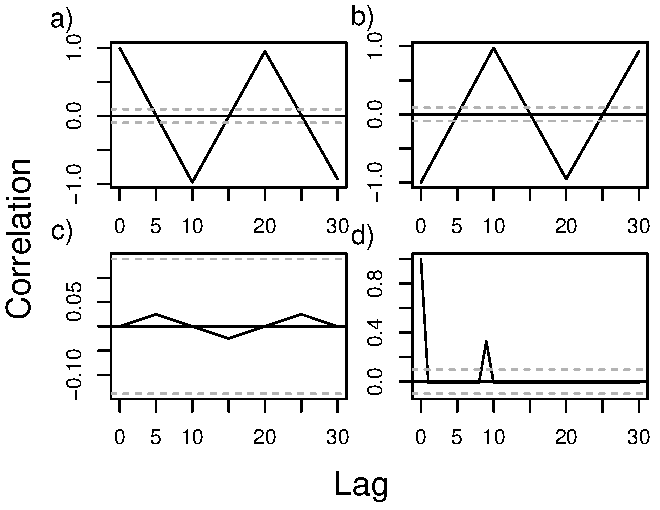
\includegraphics[width=\textwidth]{figures/example_xcorrs.pdf}
    \caption{Variation in cross-correlation values for different combinations of position histories. The extreme variety of cross-correlation patterns between two moving hosts makes the effect of correlation on indirect transmission more difficult to generalize than direct transmission.}
    \label{fig:xcorrs}
\end{figure}


\end{document}
